\chapter{RSA}
\section{Ablauf}
RSA (asymmetrisch) verwendet als Falltürfunktion die \textbf{Primzahlmultiplikation} und nutzt die Schwierigkeit der \textbf{Primfaktorzerlegung}.

\begin{figure}[H]
	\centering
	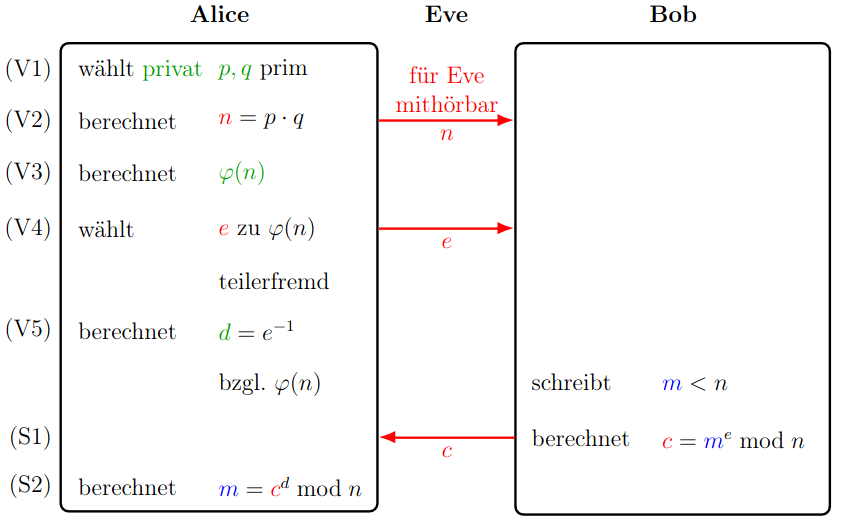
\includegraphics[width=1.0\linewidth]{figures/rsa_basic.png}
	\caption{RSA Ablauf}
\end{figure}
\begin{enumerate}[leftmargin=*,label={\textbf{V\arabic*\:}}]
	\item Es werden zwei Primzahlen $p$ und $q$ ausgewählt
	\item Modul $n$ wird berechnet, $n$ = $p$ $\cdot$ $q$, und veröffentlicht
	\item Danach wird $\varphi$($n$) berechnet, da $p$ und $q$ beide Primzahlen sind ist dies einfach: $\varphi$($n$) = ($p$ - 1) $\cdot$ ($q$ - 1)
	\item Der Verschlüsselungsexponent $e$ wird gewählt, indem eine teilerfremde Zahl zu $\varphi$($n$) ermittelt wird und wird veröffentlicht ($e$ ... \textbf{e}ncrypt).
	\item Da $e$ in $\mathbb{Z}_{\varphi(n)}$ invertierbar ist, kann man mit \textbf{erweiterten euklidischen Algorithmus} das Inverse $d$ von $e$ berechnen. $d$ gilt dann als Entschlüsselungsexponent ($d$ ... \textbf{d}ecrypt)
\end{enumerate}
\begin{enumerate}[leftmargin=*,label={\textbf{S\arabic*\:}}]
	\item Verschlüsselung von $m$ mittels $c$ = $m^e$ mod $n$
	\item Entschlüsselung von $c$ mittels $m$ = $c^d$ mod $n$
\end{enumerate}

\section{Allgemein}
RSA ist natürlich anfällig für \textbf{Chosen-Plaintext Angriffe}, da $e$ zum Verschlüsseln öffentlich ist. Lösung: großes $n$.

Angriff gegen RSA: \textbf{Faktorisierungsangriff}: Es wird versucht die Primfaktorzerlegung von $n$ zu finden. Bei 512 Bit RSA ist dieser Angriff möglich $\rightarrow$ dementsprechend mindestens 1024 Bit verwenden. 

Meist erfolgen aber Angriff über Seitenkanäle.





